
\subsection{Validation Tests Multishape}
(Note: all the things from this section are in PDECO/MultiShapeTesting in Matlab. The following files are particularly relevant:
PlottingNormalComparison, TablesExactSolutions, TableForwardExamples, TablesDiffIntetc and MultiShapeAssorted. The other files are called inside these wrappers. Plotting is currently commented out but burried in there somewhere...)

\subsubsection{Testing Differentiation, Interpolation, Convolution and Integration} \label{sec:ValidationDiffIntetc}
TablesDiffIntetc() in Matlab
	\begin{figure}[h]
	\centering
	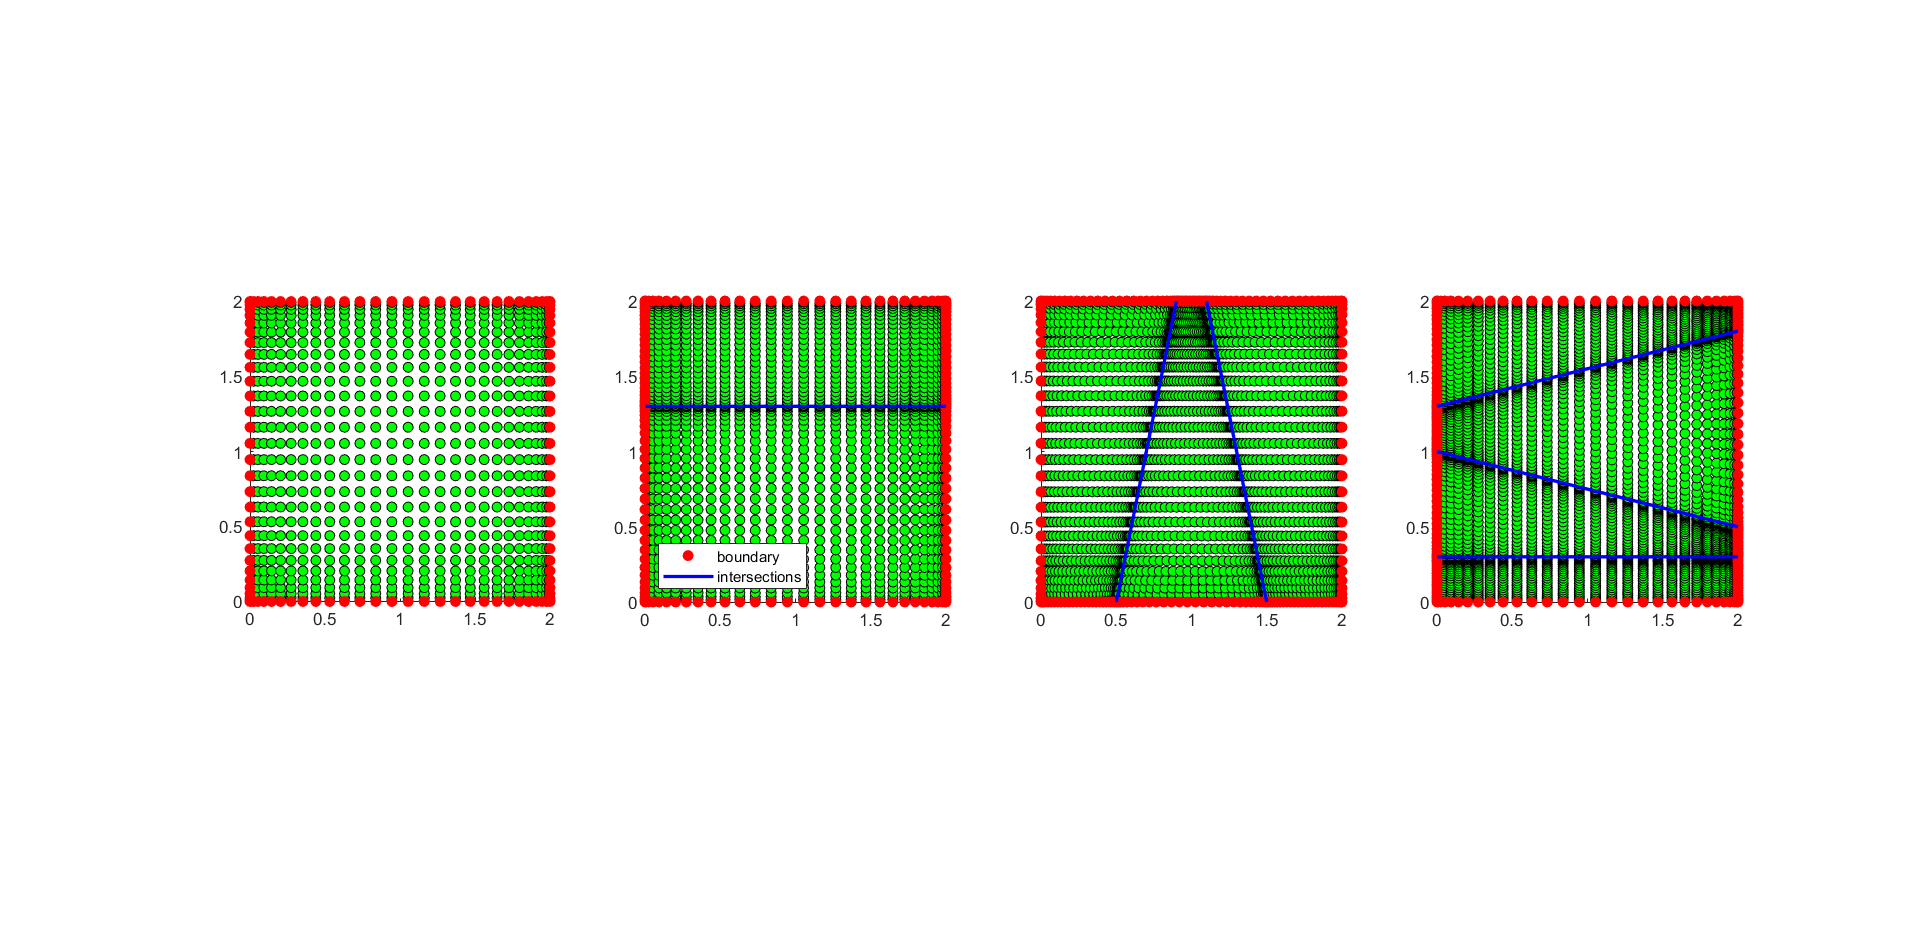
\includegraphics[scale=0.35]{BoxSections.png}
	\caption{Different discretizations of the box (a - g).} 
	\label{F2}
\end{figure}
\begin{figure}[h]
	\centering
	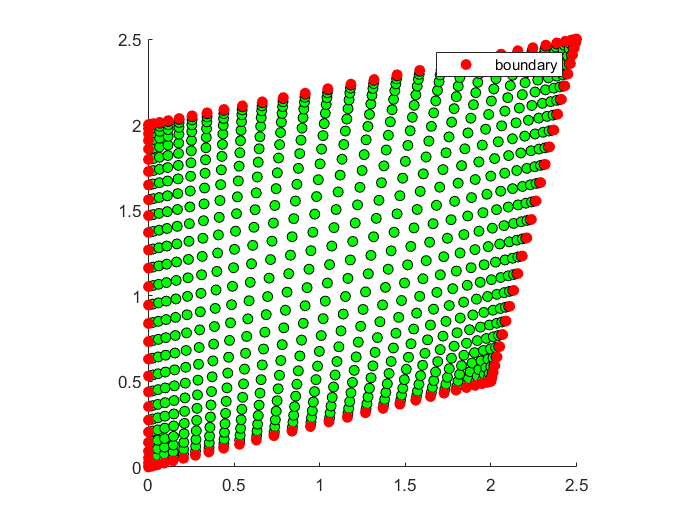
\includegraphics[scale=0.35]{quad.png}
	\caption{Quadrilateral domain (q).} 
	\label{F3a}
\end{figure}
\begin{figure}[h]
	\centering
	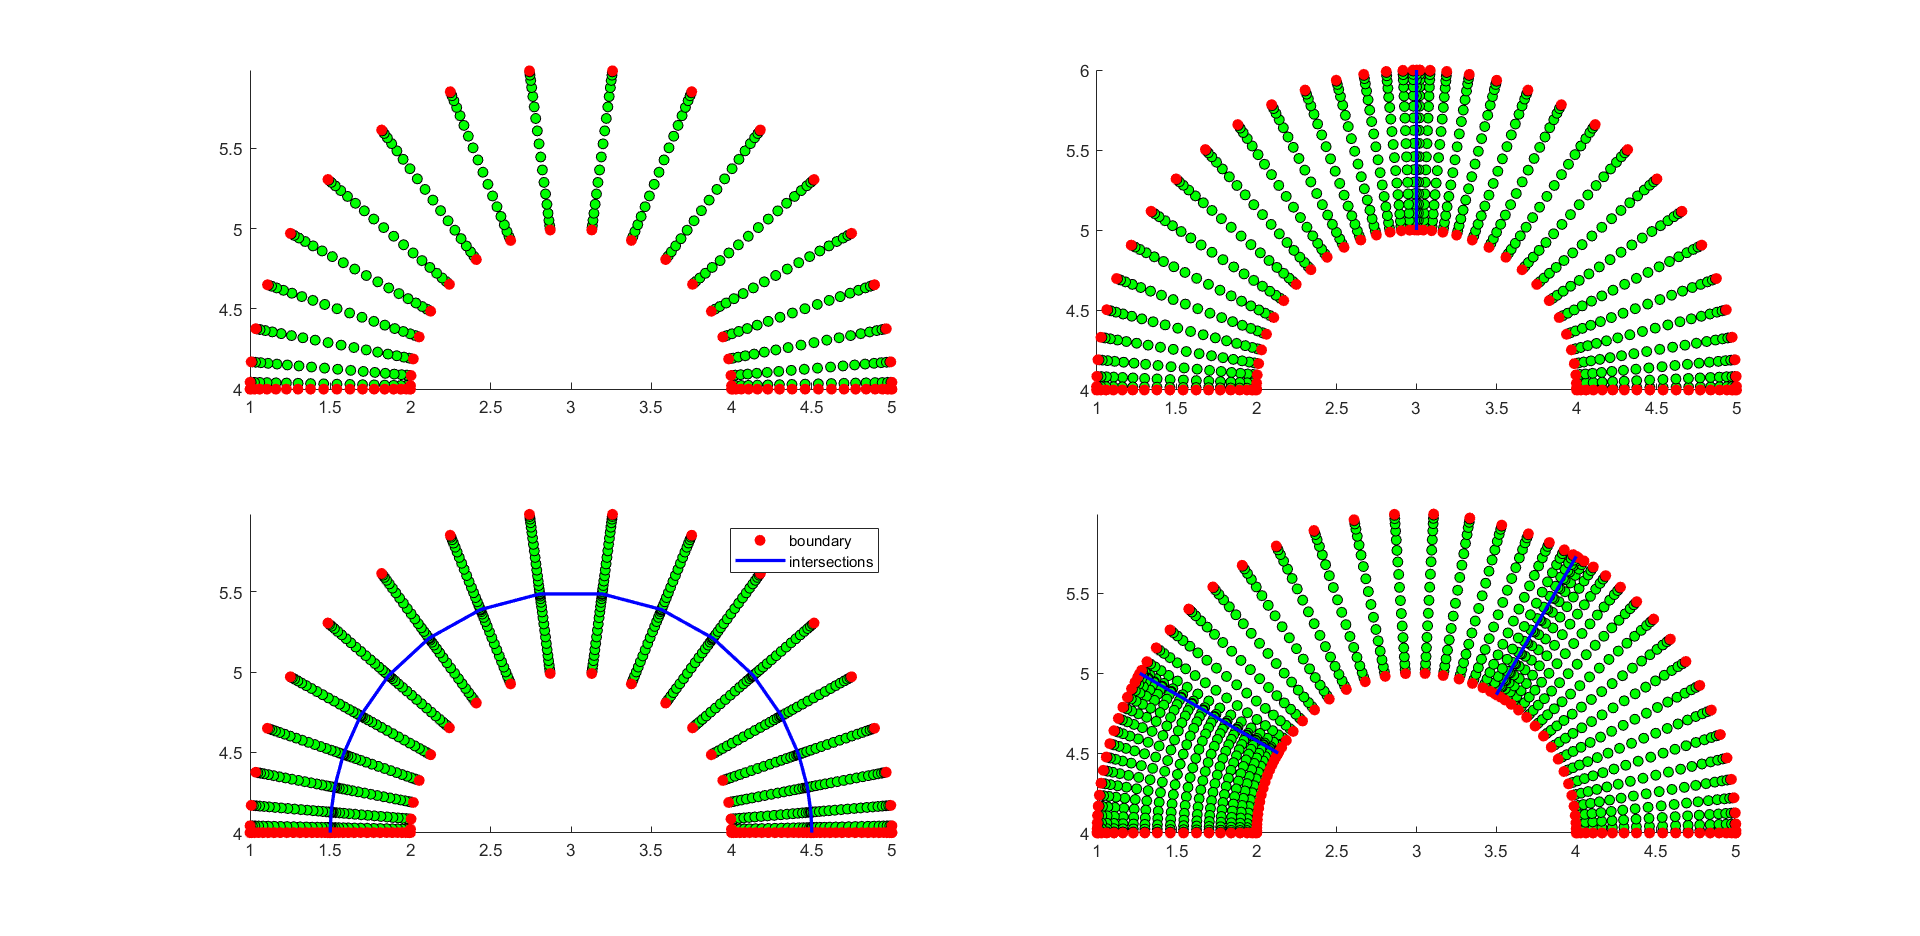
\includegraphics[scale=0.35]{WedgeSections.png}
	\caption{Different discretizations of the wedge (h - k).} 
	\label{F4}
\end{figure}


We investigate the accuracy of differentiation, interpolation, integration and convolution comparing different discretizations of the box and a wedge. The different discretizations can be seen in Figures \ref{F2}, \ref{F3a} and \ref{F4}.
The operations are validated using the exact solution
\begin{align}\label{eq:exactsol1}
	\rho &= \exp( \alpha_1  t + \beta_1 y_1 + \beta_2 y_2),\\
	\nabla \rho &= [\beta_1 \rho, \beta_2 \rho],\notag \\
	\nabla^2 \rho &= \nabla \cdot \nabla \rho = (\beta_1^2 + \beta_2^2)\rho,\notag
\end{align}
where $	\beta_1 = 0.1 $, $\beta_2 = 0.1$, $\alpha_1 = -0.5$.


We test each of the operators $\Grad$, $\Div$ and $\Lap$ by computing the error between the numerical and the exact solution
\begin{align}\label{eq:ErrorMeasure1}
	\mathcal E_{\text{Abs}} (f)&= \max \max \abs{f_{num} - f_{ex}}\\
	\mathcal E_{\text{Rel}} (f)&= \frac{\mathcal E_{\text{Abs}}(f) }{ \max \max \abs{f_{ex}}}.
\end{align}
The $\Div$ operator is tested by taking the divergence of the exact solution for $\nabla \rho$ and comparing it to the exact solution for $\nabla^2 \rho$. Note that the exact $\nabla \rho$ has to be transformed into polar coordinates first. The solutions can be seen in Tables \ref{Tab:Grad}, \ref{Tab:div} and \ref{Tab:Lap}.

We investigate the functionality of the interpolation matrix by interpolating from the different multishapes onto a uniform grid. This grid is created by setting up a uniform rectangular grid which fully contains the multishape. Then we loop through the shapes and interpolate the test function $\rho$ \eqref{eq:exactsol1} onto the uniform points that lie inside each shape. In the end we discard the points that lie outside the multishape. This causes the final solution on the uniform grid to vary in size, depending on the discretization of the multishape. We test the functionality by comparing the interpolated function values to $\rho$ evaluated on the uniform grid points, using \eqref{eq:ErrorMeasure1}. The results can be seen in Table \ref{Tab:Interp}.

In a second test we interpolate a function $\rho$, \eqref{eq:exactsol1}, computed with $N =50$ on shapes (a) and (h) respectively onto a uniform grid, as described above. Then we compute \eqref{eq:exactsol1} on the multishapes (b), (f), and (g) with $N = 10$, $N = 20$ and $N = 30$. We interpolate this onto the same uniform grid as shape (a) using the physical interpolation function. The values of $\rho$ coming from (a) can be compared with those from (b), (f), and (g) on the uniform grid, using (a) as a reference solution. Similarly, the solution on shape (h) serves as reference solution for multishapes (j) and (k). The errors, computed using \eqref{eq:ErrorMeasure1} can be seen in Table \ref{Tab:InterpComp}.

Finally, we investigate what happens when we consider interpolation to a uniform grid with $N_1 \neq N_2$ for the wedge, when compared to the exact solution on the uniform grid. This is interesting, because when the solution is interpolated onto a uniform grid (in Cartesian coordinates), it is to be expected that more points are needed in the angular direction than in the radial direction, since in Cartesian coordinates points are more densely clustered in radial direction, as can be seen in Figure \ref{F4}. This is indeed what happens, as can be seen in Table \ref{Tab:InterpPol}. We get considerably better results for small $N_1$ than for small $N_2$ and vice versa. We could investigate whether this behaviour changes when we choose a shape with small angle and long radius instead.

We consider a similar approach for testing the convolution matrix. We compute the convolution matrix with $N = 50$ on shape (a) (or (h) respectively) and apply it to the function $\rho$ in equation \eqref{eq:exactsol1}. We then interpolate this onto the other shapes and compute the error \eqref{eq:ErrorMeasure1} with the convolution of $\rho$ on that shape. We use the value of the convolution on a single shape with $N = 50$ as the reference value for the multishape convolution. The results are displayed in Table \ref{Tab:Conv}.

For the integration vector, we compute the integral of $\rho$ on shape (a) and compare this to the integral of $\rho$ on multishapes (b), (f) and (g). We then compare the integral of $\rho$ on the single shape (h) to the one on discretizations (j) and (k). The errors computed with \eqref{eq:ErrorMeasure1} can be seen in Table \ref{Tab:Int}, where again the value of the integral on the single shape is the reference for the multishape integration.
\begin{table}
\centering
\begin{tabular}{ | c | c | c | c | c | c | c |}
\hline
 & \multicolumn{2}{c|}{$N = 10$}  & \multicolumn{2}{c|}{$N = 20$}  & \multicolumn{2}{c|}{$N = 30$} \\
\hline
 & $\mathcal E_{Abs}$ & $\mathcal E_{Rel}$ & $\mathcal E_{Abs}$ & $\mathcal E_{Rel}$ & $\mathcal E_{Abs}$  & $\mathcal E_{Rel}$ \\
\hline
 a & $\numprint{3.6637e-15}$ & $\numprint{4.0491e-14}$ & $\numprint{4.5158e-14}$ & $\numprint{4.9908e-13}$ & $\numprint{1.0987e-13}$ & $\numprint{1.2143e-12}$ \\
 b & $\numprint{2.5202e-14}$ & $\numprint{2.7853e-13}$ & $\numprint{1.3006e-13}$ & $\numprint{1.4374e-12}$ & $\numprint{3.9264e-13}$ & $\numprint{4.3394e-12}$ \\
 c & $\numprint{3.5680e-14}$ & $\numprint{3.9432e-13}$ & $\numprint{2.7724e-13}$ & $\numprint{3.0639e-12}$ & $\numprint{1.0356e-12}$ & $\numprint{1.1445e-11}$ \\
 d & $\numprint{7.3080e-14}$ & $\numprint{8.0766e-13}$ & $\numprint{6.0429e-13}$ & $\numprint{6.6785e-12}$ & $\numprint{1.2559e-12}$ & $\numprint{1.3880e-11}$ \\
 e & $\numprint{3.1912e-14}$ & $\numprint{3.5268e-13}$ & $\numprint{2.0508e-13}$ & $\numprint{2.2665e-12}$ & $\numprint{6.5671e-13}$ & $\numprint{7.2578e-12}$ \\
 f & $\numprint{5.7149e-14}$ & $\numprint{6.3159e-13}$ & $\numprint{4.4410e-13}$ & $\numprint{4.9081e-12}$ & $\numprint{1.7717e-12}$ & $\numprint{1.9580e-11}$ \\
 g & $\numprint{1.3947e-14}$ & $\numprint{1.5414e-13}$ & $\numprint{9.5771e-14}$ & $\numprint{1.0584e-12}$ & $\numprint{2.6459e-13}$ & $\numprint{2.9242e-12}$ \\
 h & $\numprint{3.1143e-5}$ & $\numprint{1.3588e-4}$ & $\numprint{1.3522e-11}$ & $\numprint{5.9203e-11}$ & $\numprint{4.0515e-13}$ & $\numprint{1.7705e-12}$ \\
 i & $\numprint{1.3490e-7}$ & $\numprint{5.9567e-7}$ & $\numprint{2.4433e-13}$ & $\numprint{1.0689e-12}$ & $\numprint{4.5003e-13}$ & $\numprint{1.9658e-12}$ \\
 j & $\numprint{3.1143e-5}$ & $\numprint{1.3588e-4}$ & $\numprint{1.3522e-11}$ & $\numprint{5.9203e-11}$ & $\numprint{9.8901e-13}$ & $\numprint{4.3219e-12}$ \\
 k & $\numprint{9.8299e-8}$ & $\numprint{4.2888e-7}$ & $\numprint{3.1769e-13}$ & $\numprint{1.3866e-12}$ & $\numprint{8.6467e-13}$ & $\numprint{3.7732e-12}$ \\
\hline
\end{tabular}
\caption{Table $\Grad$}
\label{Tab:Grad}
\end{table}
\begin{table}
\centering
\begin{tabular}{ | c | c | c | c | c | c | c |}
\hline
 & \multicolumn{2}{c|}{$N = 10$}  & \multicolumn{2}{c|}{$N = 20$}  & \multicolumn{2}{c|}{$N = 30$} \\
\hline
 & $\mathcal E_{Abs}$ & $\mathcal E_{Rel}$ & $\mathcal E_{Abs}$ & $\mathcal E_{Rel}$ & $\mathcal E_{Abs}$  & $\mathcal E_{Rel}$ \\
\hline
 a & $\numprint{8.3267e-16}$ & $\numprint{4.6012e-14}$ & $\numprint{4.8798e-15}$ & $\numprint{2.6965e-13}$ & $\numprint{1.2278e-14}$ & $\numprint{6.7849e-13}$ \\
 b & $\numprint{2.9594e-15}$ & $\numprint{1.6353e-13}$ & $\numprint{1.3121e-14}$ & $\numprint{7.2507e-13}$ & $\numprint{4.0837e-14}$ & $\numprint{2.2566e-12}$ \\
 c & $\numprint{8.3614e-15}$ & $\numprint{4.6204e-13}$ & $\numprint{2.8682e-14}$ & $\numprint{1.5849e-12}$ & $\numprint{1.0649e-13}$ & $\numprint{5.8845e-12}$ \\
 d & $\numprint{7.9138e-15}$ & $\numprint{4.3731e-13}$ & $\numprint{4.2664e-14}$ & $\numprint{2.3575e-12}$ & $\numprint{9.6187e-14}$ & $\numprint{5.3152e-12}$ \\
 e & $\numprint{3.6846e-15}$ & $\numprint{2.0360e-13}$ & $\numprint{2.1975e-14}$ & $\numprint{1.2143e-12}$ & $\numprint{6.9682e-14}$ & $\numprint{3.8505e-12}$ \\
 f & $\numprint{9.7717e-15}$ & $\numprint{5.3997e-13}$ & $\numprint{6.4991e-14}$ & $\numprint{3.5913e-12}$ & $\numprint{1.3360e-13}$ & $\numprint{7.3824e-12}$ \\
 g & $\numprint{3.0878e-15}$ & $\numprint{1.7063e-13}$ & $\numprint{1.0623e-14}$ & $\numprint{5.8704e-13}$ & $\numprint{3.3662e-14}$ & $\numprint{1.8601e-12}$ \\
 h & $\numprint{5.2272e-5}$ & $\numprint{1.6127e-3}$ & $\numprint{3.4844e-11}$ & $\numprint{1.0758e-9}$ & $\numprint{5.3096e-14}$ & $\numprint{1.6387e-12}$ \\
 i & $\numprint{9.2692e-8}$ & $\numprint{2.8672e-6}$ & $\numprint{3.2897e-14}$ & $\numprint{1.0155e-12}$ & $\numprint{6.4497e-14}$ & $\numprint{1.9903e-12}$ \\
 j & $\numprint{5.2272e-5}$ & $\numprint{1.6127e-3}$ & $\numprint{3.4852e-11}$ & $\numprint{1.0761e-9}$ & $\numprint{1.3768e-13}$ & $\numprint{4.2490e-12}$ \\
 k & $\numprint{8.4307e-8}$ & $\numprint{2.6010e-6}$ & $\numprint{4.5634e-14}$ & $\numprint{1.4080e-12}$ & $\numprint{9.0605e-14}$ & $\numprint{2.7954e-12}$ \\
\hline
\end{tabular}
\caption{Table $\Div$}
\label{Tab:div}
\end{table}
\begin{table}
\centering
\begin{tabular}{ | c | c | c | c | c | c | c |}
\hline
 & \multicolumn{2}{c|}{$N = 10$}  & \multicolumn{2}{c|}{$N = 20$}  & \multicolumn{2}{c|}{$N = 30$} \\
\hline
 & $\mathcal E_{Abs}$ & $\mathcal E_{Rel}$ & $\mathcal E_{Abs}$ & $\mathcal E_{Rel}$ & $\mathcal E_{Abs}$  & $\mathcal E_{Rel}$ \\
\hline
 a & $\numprint{1.7055e-13}$ & $\numprint{9.4244e-12}$ & $\numprint{4.7951e-12}$ & $\numprint{2.6497e-10}$ & $\numprint{2.5029e-11}$ & $\numprint{1.3831e-9}$ \\
 b & $\numprint{1.3937e-12}$ & $\numprint{7.7015e-11}$ & $\numprint{4.4301e-11}$ & $\numprint{2.4480e-9}$ & $\numprint{1.2869e-10}$ & $\numprint{7.1114e-9}$ \\
 c & $\numprint{7.7744e-12}$ & $\numprint{4.2960e-10}$ & $\numprint{3.8083e-10}$ & $\numprint{2.1044e-8}$ & $\numprint{3.8902e-9}$ & $\numprint{2.1497e-7}$ \\
 d & $\numprint{1.4964e-11}$ & $\numprint{8.2688e-10}$ & $\numprint{5.5707e-10}$ & $\numprint{3.0783e-8}$ & $\numprint{1.6726e-9}$ & $\numprint{9.2426e-8}$ \\
 e & $\numprint{4.2647e-12}$ & $\numprint{2.3566e-10}$ & $\numprint{1.0580e-10}$ & $\numprint{5.8462e-9}$ & $\numprint{1.0035e-9}$ & $\numprint{5.5450e-8}$ \\
 f & $\numprint{1.4029e-11}$ & $\numprint{7.7521e-10}$ & $\numprint{5.8611e-10}$ & $\numprint{3.2388e-8}$ & $\numprint{3.0143e-9}$ & $\numprint{1.6657e-7}$ \\
 g & $\numprint{9.4664e-13}$ & $\numprint{5.2310e-11}$ & $\numprint{3.5819e-11}$ & $\numprint{1.9793e-9}$ & $\numprint{1.4403e-10}$ & $\numprint{7.9586e-9}$ \\
 h & $\numprint{5.3665e-4}$ & $\numprint{1.6556e-2}$ & $\numprint{1.0457e-9}$ & $\numprint{3.2287e-8}$ & $\numprint{1.7551e-10}$ & $\numprint{5.4167e-9}$ \\
 i & $\numprint{4.6482e-6}$ & $\numprint{1.4378e-4}$ & $\numprint{5.0420e-11}$ & $\numprint{1.5565e-9}$ & $\numprint{2.3952e-10}$ & $\numprint{7.3915e-9}$ \\
 j & $\numprint{5.3665e-4}$ & $\numprint{1.6556e-2}$ & $\numprint{1.0223e-9}$ & $\numprint{3.1565e-8}$ & $\numprint{7.2370e-10}$ & $\numprint{2.2335e-8}$ \\
 k & $\numprint{3.3996e-6}$ & $\numprint{1.0488e-4}$ & $\numprint{1.0291e-10}$ & $\numprint{3.1753e-9}$ & $\numprint{4.0443e-10}$ & $\numprint{1.2478e-8}$ \\
\hline
\end{tabular}
\caption{Table $\Lap$}
\label{Tab:Lap}
\end{table}
\begin{table}
\centering
\begin{tabular}{ | c | c | c | c | c | c | c |}
\hline
 & \multicolumn{2}{c|}{$N = 10$}  & \multicolumn{2}{c|}{$N = 20$}  & \multicolumn{2}{c|}{$N = 30$} \\
\hline
 & $\mathcal E_{Abs}$ & $\mathcal E_{Rel}$ & $\mathcal E_{Abs}$ & $\mathcal E_{Rel}$& $\mathcal E_{Abs}$  & $\mathcal E_{Rel}$ \\
\hline
 a & $\numprint{9.9920e-16}$ & $\numprint{1.1043e-15}$ & $\numprint{1.1102e-15}$ & $\numprint{1.2270e-15}$ & $\numprint{1.9984e-15}$ & $\numprint{2.2086e-15}$ \\
 b & $\numprint{8.8818e-16}$ & $\numprint{9.8159e-16}$ & $\numprint{1.5543e-15}$ & $\numprint{1.7178e-15}$ & $\numprint{1.8874e-15}$ & $\numprint{2.0859e-15}$ \\
 c & $\numprint{8.8818e-16}$ & $\numprint{9.8159e-16}$ & $\numprint{1.6653e-15}$ & $\numprint{1.8405e-15}$ & $\numprint{2.2204e-15}$ & $\numprint{2.4540e-15}$ \\
 d & $\numprint{8.8818e-16}$ & $\numprint{9.8159e-16}$ & $\numprint{1.9984e-15}$ & $\numprint{2.2086e-15}$ & $\numprint{2.6645e-15}$ & $\numprint{2.9448e-15}$ \\
 e & $\numprint{8.8818e-16}$ & $\numprint{9.8159e-16}$ & $\numprint{1.4433e-15}$ & $\numprint{1.5951e-15}$ & $\numprint{2.6645e-15}$ & $\numprint{2.9448e-15}$ \\
 f & $\numprint{1.2212e-15}$ & $\numprint{1.3497e-15}$ & $\numprint{1.6653e-15}$ & $\numprint{1.8405e-15}$ & $\numprint{2.8866e-15}$ & $\numprint{3.1902e-15}$ \\
 g & $\numprint{8.8818e-16}$ & $\numprint{9.8159e-16}$ & $\numprint{1.8874e-15}$ & $\numprint{2.0859e-15}$ & $\numprint{2.5535e-15}$ & $\numprint{2.8221e-15}$ \\
 h & $\numprint{4.6655e-6}$ & $\numprint{2.8922e-6}$ & $\numprint{7.9314e-13}$ & $\numprint{4.9000e-13}$ & $\numprint{2.6645e-15}$ & $\numprint{1.6450e-15}$ \\
 i & $\numprint{1.1935e-8}$ & $\numprint{7.3650e-9}$ & $\numprint{3.3307e-15}$ & $\numprint{2.0553e-15}$ & $\numprint{3.1086e-15}$ & $\numprint{1.9183e-15}$ \\
 j & $\numprint{4.6655e-6}$ & $\numprint{2.8922e-6}$ & $\numprint{7.9226e-13}$ & $\numprint{4.8945e-13}$ & $\numprint{4.2188e-15}$ & $\numprint{2.6047e-15}$ \\
 k & $\numprint{7.7730e-9}$ & $\numprint{4.8017e-9}$ & $\numprint{2.2204e-15}$ & $\numprint{1.3705e-15}$ & $\numprint{4.4409e-15}$ & $\numprint{2.7405e-15}$ \\
\hline
\end{tabular}
\caption{Table Interp}
\label{Tab:Interp}
\end{table}
\begin{table}
\centering
\begin{tabular}{ | c | c | c | c | c | c | c |}
\hline
 & \multicolumn{2}{c|}{$N = 10$}  & \multicolumn{2}{c|}{$N = 20$}  & \multicolumn{2}{c|}{$N = 30$} \\
\hline
 & $\mathcal E_{Abs}$ & $\mathcal E_{Rel}$ & $\mathcal E_{Abs}$ & $\mathcal E_{Rel}$ & $\mathcal E_{Abs}$  & $\mathcal E_{Rel}$ \\
\hline
 b & $\numprint{2.3315e-15}$ & $\numprint{2.5767e-15}$ & $\numprint{2.3315e-15}$ & $\numprint{2.5767e-15}$ & $\numprint{3.2196e-15}$ & $\numprint{3.5583e-15}$ \\
 c & $\numprint{2.4425e-15}$ & $\numprint{2.6994e-15}$ & $\numprint{2.8866e-15}$ & $\numprint{3.1902e-15}$ & $\numprint{2.5535e-15}$ & $\numprint{2.8221e-15}$ \\
 d & $\numprint{2.3315e-15}$ & $\numprint{2.5767e-15}$ & $\numprint{3.2196e-15}$ & $\numprint{3.5583e-15}$ & $\numprint{3.3307e-15}$ & $\numprint{3.6810e-15}$ \\
 e & $\numprint{2.3315e-15}$ & $\numprint{2.5767e-15}$ & $\numprint{2.6645e-15}$ & $\numprint{2.9448e-15}$ & $\numprint{2.8866e-15}$ & $\numprint{3.1902e-15}$ \\
 f & $\numprint{2.2204e-15}$ & $\numprint{2.4540e-15}$ & $\numprint{2.7756e-15}$ & $\numprint{3.0675e-15}$ & $\numprint{3.2196e-15}$ & $\numprint{3.5583e-15}$ \\
 g & $\numprint{2.6645e-15}$ & $\numprint{2.9448e-15}$ & $\numprint{2.9976e-15}$ & $\numprint{3.3129e-15}$ & $\numprint{3.6637e-15}$ & $\numprint{4.0491e-15}$ \\
 i & $\numprint{1.1886e-8}$ & $\numprint{7.3362e-9}$ & $\numprint{5.1070e-15}$ & $\numprint{3.1520e-15}$ & $\numprint{6.4393e-15}$ & $\numprint{3.9742e-15}$ \\
 j & $\numprint{4.8940e-6}$ & $\numprint{3.0205e-6}$ & $\numprint{8.1379e-13}$ & $\numprint{5.0226e-13}$ & $\numprint{4.6629e-15}$ & $\numprint{2.8779e-15}$ \\
 k & $\numprint{7.8923e-9}$ & $\numprint{4.8710e-9}$ & $\numprint{5.1070e-15}$ & $\numprint{3.1520e-15}$ & $\numprint{5.1070e-15}$ & $\numprint{3.1520e-15}$ \\
\hline
\end{tabular}
\caption{Table Interp Compare}
\label{Tab:InterpComp}
\end{table}
\begin{table}
\centering
\begin{tabular}{ | c | c | c | c | c | c | c |}
\hline
 & $N_1 = 20$ & $N_1 = 20$& $N_1 = 5$& $N_1 = 10$& $N_1 = 30$  & $N_1 = 20$ \\
\hline
 & $N_2 = 10$ & $ N_2 = 15$ & $ N_2 = 20$ & $ N_2 = 20$ & $ N_2 = 20$  & $ N_2 = 30$ \\
\hline
 h & $\numprint{2.8922e-6}$ & $\numprint{5.1117e-10}$ & $\numprint{1.5795e-9}$ & $\numprint{4.8973e-13}$ & $\numprint{4.9000e-13}$ & $\numprint{1.5080e-15}$ \\
 i & $\numprint{7.3650e-9}$ & $\numprint{1.6031e-14}$ & $\numprint{1.5807e-9}$ & $\numprint{1.2332e-15}$ & $\numprint{1.9183e-15}$ & $\numprint{2.4663e-15}$ \\
 j & $\numprint{2.8922e-6}$ & $\numprint{5.1117e-10}$ & $\numprint{5.1835e-11}$ & $\numprint{4.8959e-13}$ & $\numprint{4.8986e-13}$ & $\numprint{1.9192e-15}$ \\
 k & $\numprint{4.8017e-9}$ & $\numprint{7.6215e-14}$ & $\numprint{1.5808e-9}$ & $\numprint{1.2334e-15}$ & $\numprint{2.4668e-15}$ & $\numprint{2.0554e-15}$ \\
\hline
\end{tabular}
\caption{Table Comparing interpolation errors on wedges, when $N_1 \neq N_2$.}
\label{Tab:InterpPol}
\end{table}
\begin{table}
\centering
\begin{tabular}{ | c | c || c | c | c | c | c ||}
\hline
 & A.E. $ N=10$ & R.E. $N=10$ & A.E. $N = 20$ & R.E. $N = 20$ & A.E. $N=30$  & R.E. $N=30$ \\
\hline
\hline
 b & $\numprint{9.1924e-8}$ & $\numprint{5.5907e-8}$ & $\numprint{7.5495e-15}$ & $\numprint{4.5500e-15}$ & $\numprint{8.2157e-15}$ & $\numprint{4.9463e-15}$ \\
 f & $\numprint{1.4109e-8}$ & $\numprint{8.5341e-9}$ & $\numprint{8.2157e-15}$ & $\numprint{4.9497e-15}$ & $\numprint{1.9984e-14}$ & $\numprint{1.2033e-14}$ \\
 g & $\numprint{1.9228e-10}$ & $\numprint{1.1579e-10}$ & $\numprint{9.7700e-15}$ & $\numprint{5.8815e-15}$ & $\numprint{1.5543e-14}$ & $\numprint{9.3564e-15}$ \\
 j & $\numprint{1.6310e-3}$ & $\numprint{6.6333e-4}$ & $\numprint{5.0919e-8}$ & $\numprint{2.0616e-8}$ & $\numprint{8.9782e-12}$ & $\numprint{3.6342e-12}$ \\
 k & $\numprint{2.7196e-6}$ & $\numprint{1.1056e-6}$ & $\numprint{1.7668e-12}$ & $\numprint{7.1588e-13}$ & $\numprint{2.9310e-14}$ & $\numprint{1.1870e-14}$ \\
\hline
\end{tabular}
\caption{Table Conv}
\label{Tab:Conv}
\end{table}
\begin{table}
\centering
\begin{tabular}{ | c | c || c | c | c | c | c ||}
\hline
 & A.E. $ N=10$ & R.E. $N=10$ & A.E. $N = 20$ & R.E. $N = 20$ & A.E. $N=30$  & R.E. $N=30$ \\
\hline
\hline
 b & $\numprint{0.0000e+00}$ & $\numprint{0.0000e+00}$ & $\numprint{4.4409e-16}$ & $\numprint{1.4937e-16}$ & $\numprint{8.8818e-16}$ & $\numprint{2.9873e-16}$ \\
 f & $\numprint{0.0000e+00}$ & $\numprint{0.0000e+00}$ & $\numprint{0.0000e+00}$ & $\numprint{0.0000e+00}$ & $\numprint{8.8818e-16}$ & $\numprint{2.9873e-16}$ \\
 g & $\numprint{0.0000e+00}$ & $\numprint{0.0000e+00}$ & $\numprint{4.4409e-16}$ & $\numprint{1.4937e-16}$ & $\numprint{8.8818e-16}$ & $\numprint{2.9873e-16}$ \\
 j & $\numprint{2.4085e-8}$ & $\numprint{3.7621e-9}$ & $\numprint{1.7764e-15}$ & $\numprint{2.7746e-16}$ & $\numprint{2.6645e-15}$ & $\numprint{4.1620e-16}$ \\
 k & $\numprint{2.7334e-11}$ & $\numprint{4.2695e-12}$ & $\numprint{1.7764e-15}$ & $\numprint{2.7746e-16}$ & $\numprint{1.7764e-15}$ & $\numprint{2.7746e-16}$ \\
\hline
\end{tabular}
\caption{Table Int}
\label{Tab:Int}
\end{table}

